\subsubsection{Поиск событийных участков}
\paragraph{Постановка задачи}
Рассматриваются данные горизонтальной скважины X45: датчики глубины, расходомера, температуры, влагомера и два канала пассивной акустической шумометрии – низкочастотный (0-2кГц) и высокочастотный (3-32кГц). Имеется порядка 10000 точек, записанных с шагом 0.1м по глубине скважины.
Ставится задача по имеющимся данным автоматически локализовать «событийные» участки – то есть те, на которых наблюдается отклик нескольких датчиков одновременно, что может указывать на наличие зоны притока или другие события в скважине.

Используемые для анализа данные показаны на планшете на рис.\ref{fig:data}.

\begin{figure}[H]
\centering
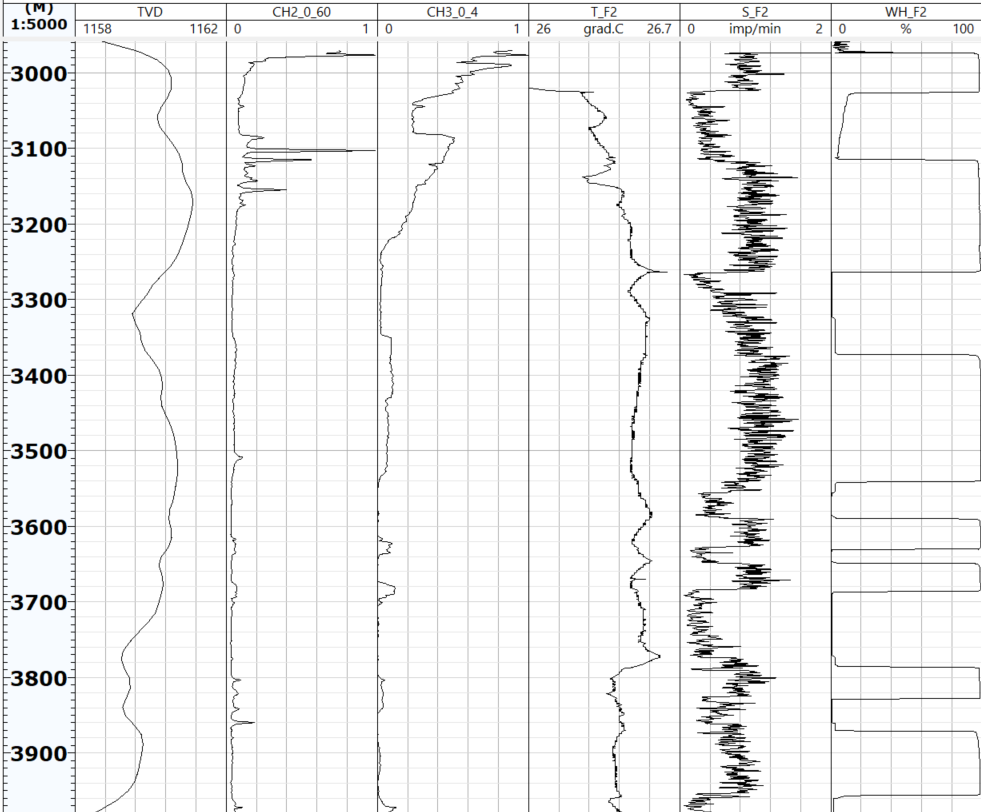
\includegraphics[width=1.0\textwidth]{WS/data.png}
\caption{Данные скважины 0X, используемые для анализа. Слева направо: показания глубины скважины, высокочастотной шумометрии, низкочастотной шумометрии, температуры, расходометрии и влагомера.}
\label{fig:data}
\end{figure}

\paragraph{Методы}
\par
Нужно локализовать отклики во всех доступных сигналах, а затем совместить их в одну разметку. Отклики могут быть несогласованы между собой различными способами:
\begin{itemize}
    \item В какой-то точке траектории есть отклики всех датчиков, кроме одного – например, в этой точке событие было, но слабое, и одному датчику не хватило чувствительности
    \item В какой-то точке траектории нет никаких откликов, кроме отклика одного датчика – например, в этой точке нет никакого значимого события, но один датчик чересчур чувствительный, и показания изменились «на пустом месте»
    \item В какой-то точке траектории часть датчиков показала отклик, а часть «промолчала» – и на первый взгляд нет однозначного решения по поводу того, каким показаниям стоит доверять.
\end{itemize}
\par
Для решения задачи, усложненной такими обстоятельствами, подойдет модель слабого контроля, описанная выше. 
\par
В выбранной терминологии, для каждого датчика можно подобрать одну или больше функций разметки – то есть экспертных правил, которые позволяют предположить, произошло на данном участке какое-то событие или нет. Функция разметки в данной постановке задачи должна выдавать один из трех ответов на каждый интервал траектории: «есть событие» (метка 1), «нет события» (метка -1), «недостаточно информации для принятия решений» (метка 0). 
\par
Здесь используем по одной функции разметки на каждый датчик. Поскольку тренды профилей для разных датчиков могут иметь разные координаты точек перелома для одного и того же события (да и событие имеет некоторую протяженность), вводится некоторое окно, которому эта метка присваивается. В данном случае окно имеет размер в 50 точек (5м). Т.е., «непрерывная» траектория при разметке заменяется на интервалы с метками через каждые 5 метров.
\par
В качестве индикатора события для расходомера, влагомера, показаний температуры и шумометрии хорошо подходят характеристики кусочно-разрывных профилей, описанных в предыдущей главе. Перед вычислением меток из всех сигналов – расходомера, влагомера, показаний датчика температуры и двух каналов шумометрии – выделяются кусочно-разрывные профили. Таким образом, для каждого сигнала у нас есть набор точек перелома, значения профиля и остаточного сигнала.
\par
Получается:
\begin{itemize}
    \item Для расходомера: считаем, что произошло событие (метка 1), если в окне находится хотя бы одна точка перелома; иначе – метка 0
    \item Для влагомера: метка 1, если в окне находится хотя бы одна точка перелома, иначе – метка 0
    \item Для температуры: метка 1, если в окне находится хотя бы одна точка, модуль значения остаточного сигнала превышает заданное значение, иначе – метка 0. Так как сигнал ввиду низкой вариативности значений практически ступенчатый, перед выделением точек перелома он был аппроксимирован сплайнами третьей степени.
    \item Для низкочастотного шума: метка 1, если в окне находится хотя бы одна точка перелома, иначе – метка 0
    \item Для высокочастотного шума: метка 1, если в окне находится хотя бы одна точка, модуль значения остаточного сигнала превышает заданное значение, иначе – метка 0.
\end{itemize}
	
\par
Указанные функции выдают только положительные либо нейтральные метки. С другой стороны, показания датчика глубины позволяют присвоить некоторым точкам отрицательные метки – то есть увеличить вероятность того, что данная точка не содержит интересующего нас события. Некоторые изменения показаний датчиков могут являться исключительно следствием влияния траектории – например, вода может накапливаться на вогнутых по отношению к горизонту участках траектории, что вызовет скачок влагомера, который нас не интересует. Поэтому вводится еще одна функция разметки:
\begin{itemize}
    \item Для траектории: метка -1, если внутри окна максимальное отклонение значений траектории от среднего значения внутри окна превышает $1.5 \sigma$ стандартных отклонений значений траектории по всей глубине скважины (внутри данного окна наблюдается большая, чем в среднем, осцилляция значений), иначе 0.
\end{itemize}
\par
Мы реализовали эту процедуру для траектории, но требуются дальнейшие исследования по повышению надежности такой разметки, поэтому здесь эти результаты не приводятся. 

\paragraph{Результаты}

На рисунках \ref{fig:lfs_signals} и \ref{fig:lfs_dpls} представлены предложенные функции разметки и результат обучения модели. Результаты работы разметочных функций – по одной на каждый датчик – пронумерованы как $\lambda_1, ..., \lambda_5$ и расположены справа от соответствующих датчиков. На рис.\ref{fig:lfs_signals} серым изображены изначальные сигналы; на рис.\ref{fig:lfs_dpls} – извлеченные из них профили для анализа.

\begin{figure}[H]
\centering
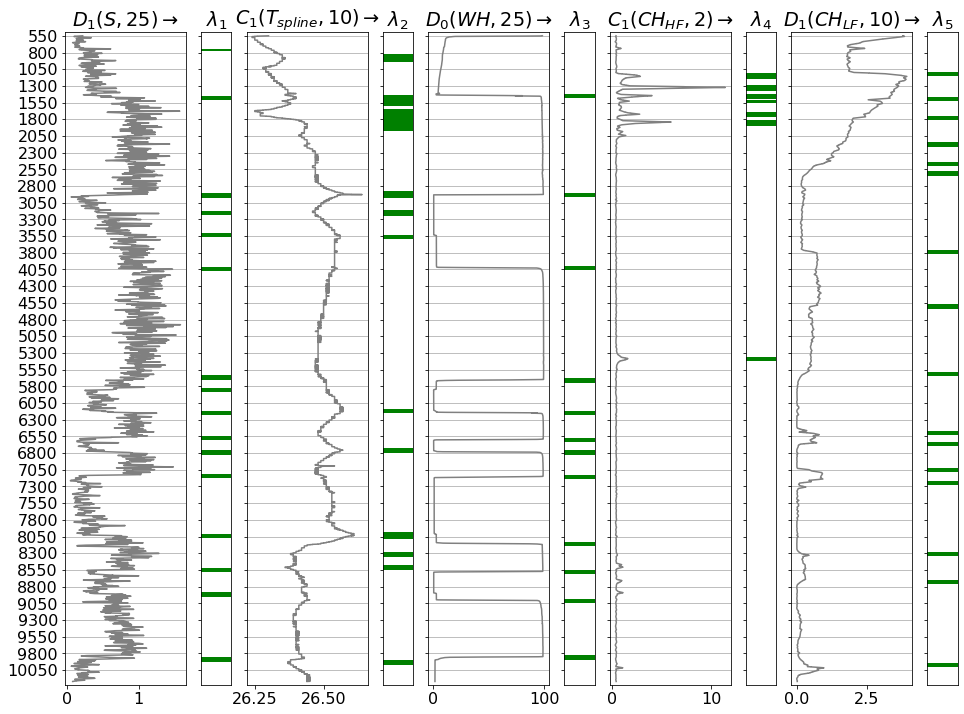
\includegraphics[width=0.8\textwidth]{WS/lfs_signals.png}
\caption{Разметочные функции, используемые для создания итоговой разметки. Серым показаны сигналы, на основе которых построены разметочные функции, зеленым выделены диапазоны, где соответствующие разметочные функции отметили вероятность события.}
\label{fig:lfs_signals}
\end{figure}

\begin{figure}[H]
\centering
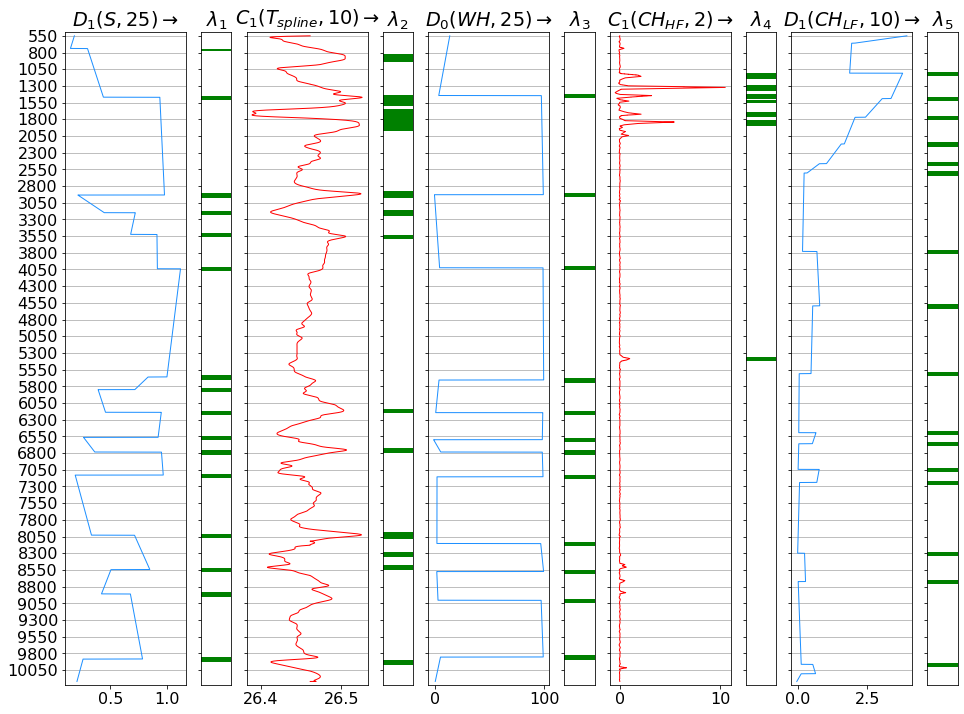
\includegraphics[width=0.8\textwidth]{WS/lfs_dpls.png}
\caption{Разметочные функции совпадают с указанными на предыдущем рисунке, но для демонстрации вместо оригинальных сигналов нарисованы выделенные профили (голубой цвет) или остаточные сигналы (красный цвет).}
\label{fig:lfs_dpls}
\end{figure}

\par
Результат работы модели – вероятностная разметка на два класса $P_{WS}$, которую можно преобразовать в дискретную разметку на два класса (1 или 0) или оставить так для оценки неопределенности. 
\par
На рисунках \ref{fig:results_optimal}, \ref{fig:results_narrow} и \ref{fig:results_wide} показаны результаты работы модели при различных параметрах минимального расстояния между событиями (значения указаны в скобках в метрах; точки разнесены на расстояние 0.1м). Первый результат предлагается считать оптимальным, следующие два получены при вариации минимального расстояния между событиями с уменьшением (\ref{fig:results_narrow}) и увеличением (\ref{fig:results_wide}) всех значений. Видно, что от этого функции разметки становятся более или менее шумными – срабатывает детекция ложных событий или наоборот, важные события оказываются пропущены. Тем не менее, общий вид итоговой разметки примерно сохраняется. Это объясняется тем, что показания температуры и высокочастотной шумометрии анализируются по значениям остатка после выделения профиля, а расходомера, влагомера и низкочастотной шумометрии – по выделенным точкам перелома. Таким образом, при увеличении минимального интервала между событиями уменьшается количество точек перелома, но становятся более шумными остатки; и наоборот – при уменьшении минимального интервала между событиями количество точек перелома увеличивается, но остатки температуры и высокочастотной шумометрии показывают меньше информации. 
\par
На рисунках \ref{fig:results_optimal}, \ref{fig:results_narrow} и \ref{fig:results_wide} класс 0 («недостаточно информации») изображен белым цветом, класс 1 («вероятно событие») - зеленым.


\begin{figure}[H]
\centering
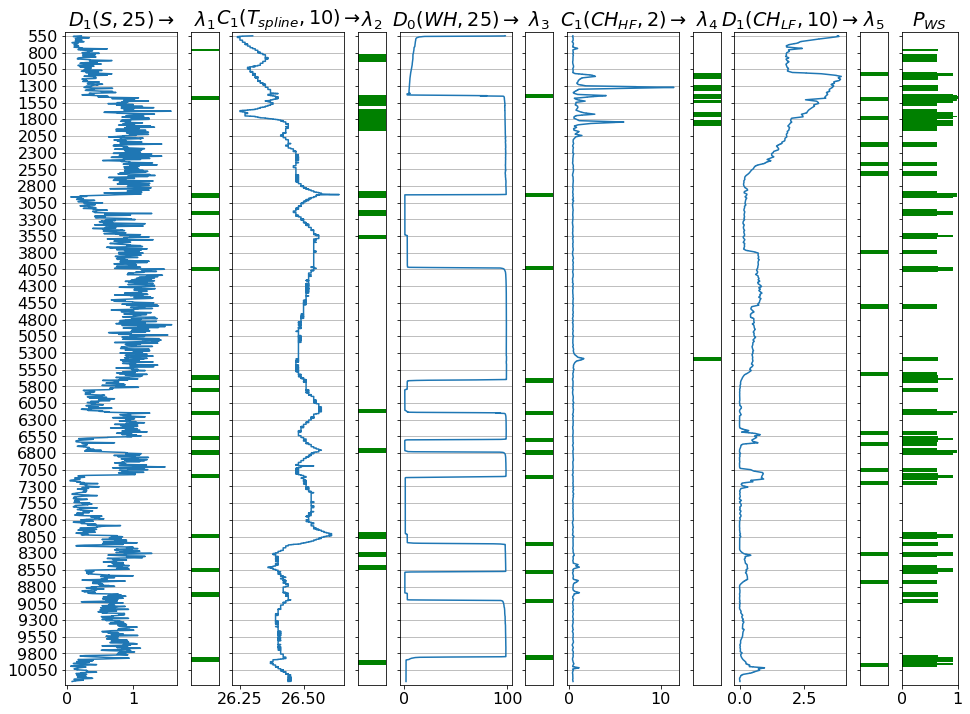
\includegraphics[width=1.0\textwidth]{WS/results_optimal.png}
\caption{Из разметочных функций в результате работы модели слабого контроля создается финальная разметка в последней колонке. Длина столбиков отражает вероятность события в данной точке.}
\label{fig:results_optimal}
\end{figure}

\par
Здесь показан результат работы модели (последний столбец $P_{WS}$) для участка в 1500 точек в приближении. 

\begin{figure}[H]
\centering
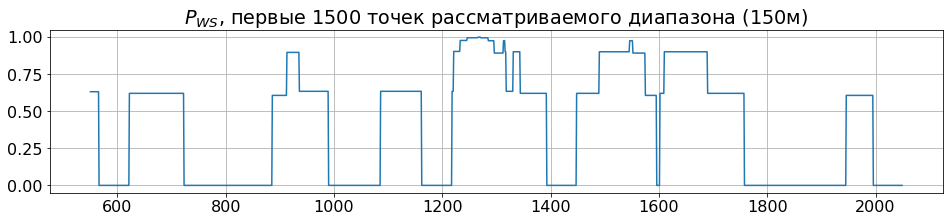
\includegraphics[width=1.0\textwidth]{WS/probability_flat.png}
\caption{Увеличенный участок последней колонки с предыдущего рисунка.}
\label{fig:probability_flat}
\end{figure}

\begin{figure}[H]
\centering
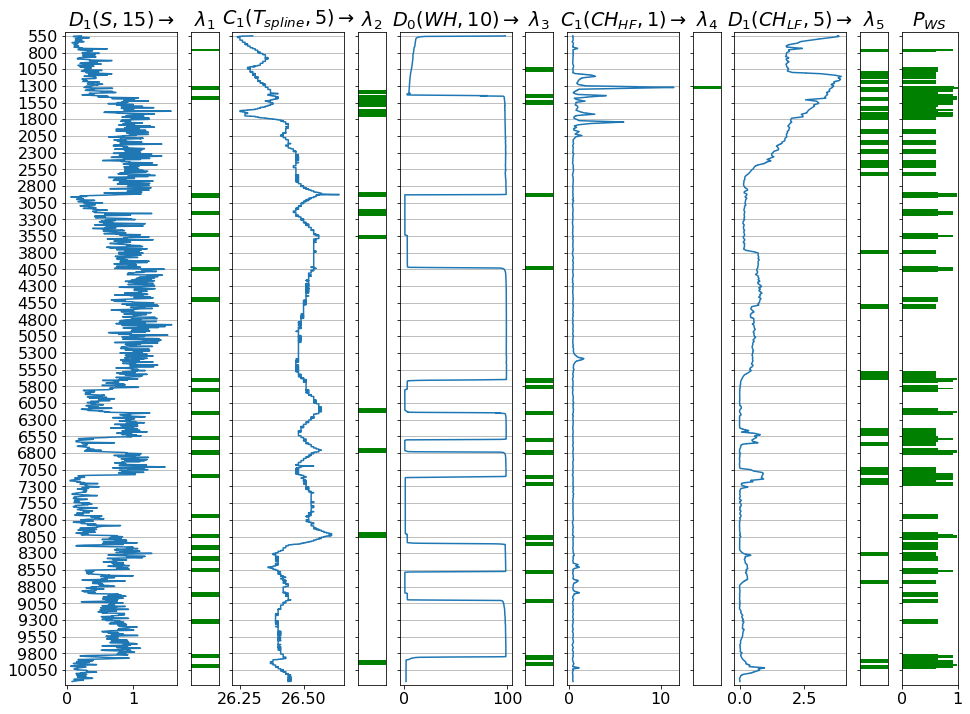
\includegraphics[width=0.8\textwidth]{WS/results_narrow.png}
\caption{Проверка устойчивости модели: для каждой разметочной функции минимальная ширина между событиями для выделения профилей была уменьшена. Видно, что финальная разметка изменилась, но не сильно.}
\label{fig:results_narrow}
\end{figure}

\begin{figure}[H]
\centering
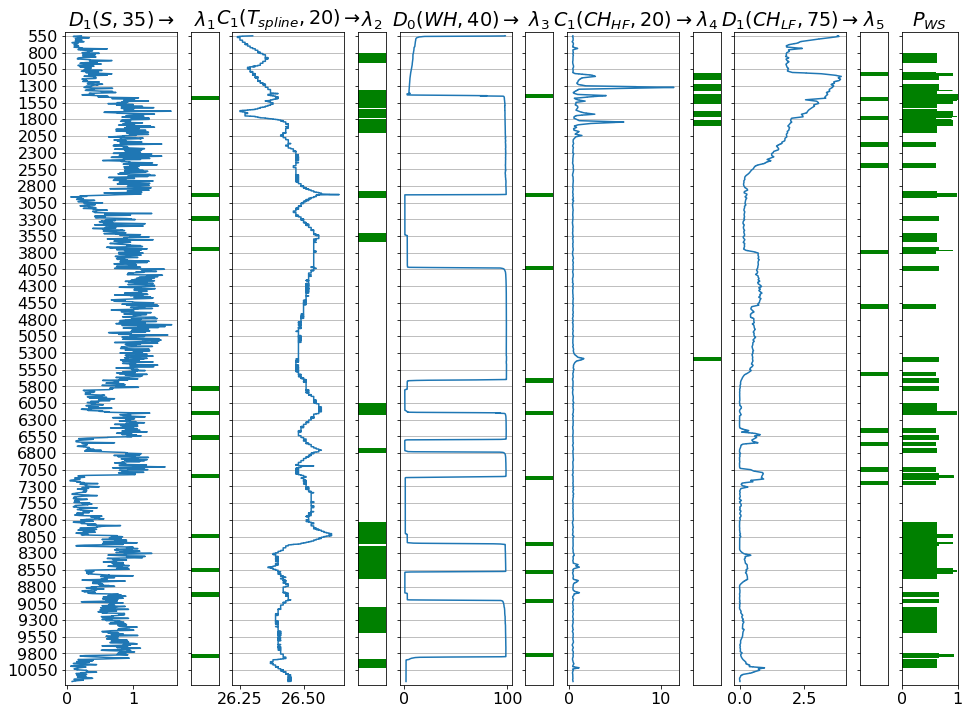
\includegraphics[width=0.8\textwidth]{WS/results_wide.png}
\caption{Аналогично предыдущему рисунку, но значения минимальной ширины между событиями были увеличены относительно оптимальных, а не уменьшены.}
\label{fig:results_wide}
\end{figure}
















